\documentclass[twoside,11pt,a4paper]{article}

\usepackage[utf8]{inputenc}
\usepackage{amsmath, amssymb, latexsym}
\usepackage{sidecap}

\usepackage{tikz}
\usetikzlibrary{decorations.pathreplacing}

\begin{document}

\begin{SCfigure}[2\sidecaptionrelwidth][t]
	\centering
	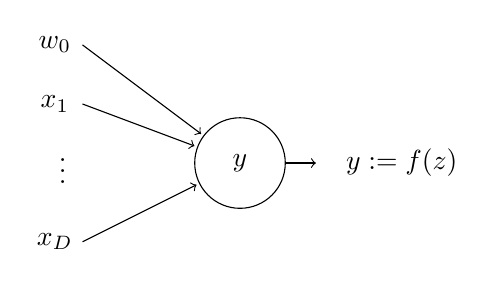
\begin{tikzpicture}[shorten >=1pt,->]
		\tikzstyle{unit}=[draw,shape=circle,minimum size=1.15cm]

		\node[unit](p) at (2,1){$y$};
		\node(dots) at (-0.25,1){\vdots};

		\draw (0,2.5) node[xshift=-10]{$w_0$} -- (p);
		\draw (0,1.75) node[xshift=-10]{$x_1$} --(p);
		\draw (0,0) node[xshift=-10]{$x_D$} -- (p);
		\draw (p) -- (3,1) node[xshift=30]{$y := f(z)$};
	\end{tikzpicture}
	\caption[Single processing units and its components.]{Single processing unit and its components. The activation function is denoted by $f$ and applied on the actual input $z$ of the unit to form its output $y = f(z)$. $x_1, \ldots, x_D$ represent input from other units within the network; $w_0$ is called bias and represents an external input to the unit. All inputs are mapped onto the actual input $z$ using the propagation rule.}
	\label{fig:processing-unit}
\end{SCfigure}

\end{document}